\section{Solve \kSUM using only \SmallO{n}-linear Queries}

We have seen that using Meiser's algorithm one can solve the \kSUM problem
with \BigO{n^3 \log^3 n} queries. During the construction of the simplex we
need at each step of this algorithm, we use projection operations on
the input point and the query hyperplanes. It is thus possible that some query we perform
involves up to \(n\) linear terms of the input.
We show that we can restrict ourselves to
\SmallO{n}-linear queries with the addition of a factor \(n\) to the complexity
of the algorithm.

\begin{figure}
\centering
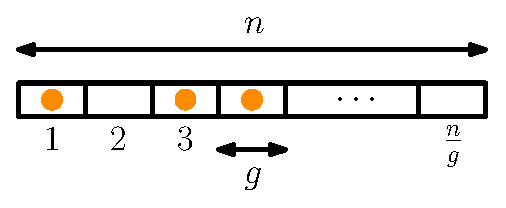
\includegraphics[width=0.4\textwidth]{fig/point-location/blocks}
\caption{Solving \kSUM for blocks \(1\), \(3\), and \(4\) only.}
\label{fig:point-location:on:blocks}
\end{figure}

We look at \ref{fig:point-location:on:blocks}. We represent input set \(\S\)
using a vector \(\enum{x_1,\ldots,x_n}\) of size \(n\). The trick is the
following. Instead of using Meiser's algorithm once to solve the problem of
size \(n\), we divide the input vector in blocks of size \(g\) and solve a
\kSUM problem for all combinations of \(k\) blocks. There are \(\sfrac{n}{g}\)
such blocks hence the number of problems to solve is \(\binom{\sfrac{n}{g}}{k}
= \BigO{(\frac{n}{g})^k} \).

The complexity of solving all the problems is thus
\begin{displaymath}
O\mleft(\group{\frac{n}{g}}^k (kg)^3 \log^3 (kg)\mright)
\end{displaymath}

Since a query can only involve elements contained in the union of \(k\)
disjoint subsets of size \(g\), the queries made are \((kg)\)-linear. Below is
a pseudo-code description of the algorithm.
\begin{algorithm}[Parameterizable \kSUM algorithm]
\item[input] Set \(\S\).
\item[1.] Partition \(\S\) into disjoint subsets
\(\S_1,\ldots,\S_{\ceil{\frac{n}{g}}}\) of size at most \(g\).
\item[2.] For each of the \(\binom{\ceil{\sfrac{n}{g}}}{k}\) possible ways to
choose \(k\) subsets \(\S_{i_1},\ldots,\S_{i_k}\) of \(\S\) without
replacement:
\item[2.1.] Solve a \kSUM instance with input \(\S_{i_1} \cup \cdots \cup
\S_{i_k}\) using Meiser's algorithm.
\item[2.2.] If the run of Meiser's algorithm yields a solution, output that
solution and stop.
\end{algorithm}

We want to parameterize \(g\) so that the queries are \SmallO{n}-linear. A
possible solution is to choose \(g = n^{\frac{k-1}{k}} = n^{1-\frac{1}{k}}\).
With this parameterization, the queries become \((kn^{1-\frac{1}{k}})\)-linear
and we obtain a complexity of
\begin{displaymath}
\BigO{n (kn^{1-\frac{1}{k}})^3 \log^3 (kn^{1-\frac{1}{k}}) }.
\end{displaymath}

Note that for any \(\alpha < k\) if we choose \(g = n^{\frac{k-\alpha}{k}} =
n^{1-\frac{\alpha}{k}}\) we end up with \((kn^{1-\frac{\alpha}{k}})\)-linear
queries and a total complexity of
\BigO{n^{\alpha} (kn^{1-\frac{\alpha}{k}})^3
\log^3 (kn^{1-\frac{\alpha}{k}}) }.
Like the lower bound given by \citet*{ailon:2005}, it gives us a
``parameterizable trade-off''
between time-complexity and query-complexity.
